\documentclass[bachelor, och, assignment]{SCWorks}
% параметр - тип обучения - одно из значений:
%    spec     - специальность
%    bachelor - бакалавриат (по умолчанию)
%    master   - магистратура
% параметр - форма обучения - одно из значений:
%    och   - очное (по умолчанию)
%    zaoch - заочное
% параметр - тип работы - одно из значений:
%    referat    - реферат
%    coursework - курсовая работа (по умолчанию)
%    diploma    - дипломная работа
%    pract      - отчет по практике
%    pract      - отчет о научно-исследовательской работе
%    autoref    - автореферат выпускной работы
%    assignment - задание на выпускную квалификационную работу
%    review     - отзыв руководителя
%    critique   - рецензия на выпускную работу
% параметр - включение шрифта
%    times    - включение шрифта Times New Roman (если установлен)
%               по умолчанию выключен
\usepackage[T2A]{fontenc}
\usepackage[utf8]{inputenc}
\usepackage{graphicx}

\usepackage[sort,compress]{cite}
\usepackage{amsmath}
\usepackage{amssymb}
\usepackage{amsthm}
\usepackage{fancyvrb}
\usepackage{longtable}
\usepackage{listings}
\usepackage{array}
\usepackage[english,russian]{babel}
\usepackage{minted}
\usepackage{tempora}

\usepackage[colorlinks=true]{hyperref}

\lstset{
    language=Python,
    numbers=left,
    backgroundcolor=\color{white},
    basicstyle=\ttfamily\footnotesize,
    breaklines=true,
    frame=none,
    tabsize=4,
    xleftmargin=0pt,
    xrightmargin=0pt,
    aboveskip=0pt,
    belowskip=0pt
}

\newcommand{\eqdef}{\stackrel {\rm def}{=}}

\newtheorem{lem}{Лемма}

\begin{document}


% Кафедра (в родительном падеже)
\chair{математической кибернетики и компьютерных наук}

% Тема работы
\title{Проект. Приложение 'Блогикум' }

% Курс
\course{2}

% Группа
\group{251}

% Факультет (в родительном падеже) (по умолчанию "факультета КНиИТ")
%\department{факультета КНиИТ}

% Специальность/направление код - наименование
\napravlenie{09.03.04 "--- Программная инженерия}
%\napravlenie{02.03.01 "--- Математическое обеспечение и администрирование информационных систем}
%\napravlenie{09.03.01 "--- Информатика и вычислительная техника}
%\napravlenie{09.03.04 "--- Программная инженерия}
%\napravlenie{10.05.01 "--- Компьютерная безопасность}

% Для студентки. Для работы студента следующая команда не нужна.
%\studenttitle{Студентки}

% Фамилия, имя, отчество в родительном падеже
\author{Архипова Ивана Сергеевича}

% Заведующий кафедрой
\chtitle{к.\,ф.-м.\,н.} % степень, звание
\chname{С.\,В.\,Миронов}

%Научный руководитель (для реферата преподаватель проверяющий работу)
\satitle{доцент, к.\,ф.-м.\,н.} %должность, степень, звание
\saname{И.\,А.\,Батраева}

% % Руководитель практики от организации (только для практики,
% % для остальных типов работ не используется)
% \patitle{к.\,ф.-м.\,н., доцент}
% \paname{Д.\,Ю.\,Петров}

% Семестр (только для практики, для остальных
% типов работ не используется)
\term{2}

% Наименование практики (только для практики, для остальных
% типов работ не используется)
\practtype{учебная}

% Продолжительность практики (количество недель) (только для практики,
% для остальных типов работ не используется)
\duration{3}

% Даты начала и окончания практики (только для практики, для остальных
% типов работ не используется)
\practStart{30.11.2025}
\practFinish{21.12.2025}

% Год выполнения отчета
\date{2025}

\maketitle


\section{Цель работы. Постановка задачи}

\textbf{Цель работы:} доработка приложения «Блогикум» по заданию из урока №4 темы №5.


\textbf{Постановка задачи:} необходимо реализовать следующие функциональные возможности:

\begin{enumerate}
    \item Кастомные страницы для ошибок (403, 404, 500).
    \item Работа с пользователями. Подключить к проекту пользователей. Создать страницу \texttt{auth/registration/} с формой для регистрации пользователей. Создать страницу пользователя.
    \item Пагинация. Подключить к проекту пагинацию и настроить вывод не более 10 публикаций: на главную страницу, на страницу пользователя, на страницу категории.
    \item Изображения к постам. Добавить возможность прикреплять изображение к публикациям проекта. Если изображение добавлено, то оно должно отображаться в публикациях на главной странице, странице пользователя, странице категории, отдельной странице публикации.
    \item Добавление новых публикаций. У зарегистрированных пользователей должна быть возможность самостоятельно публиковать посты.
    \item Редактирование публикаций.
    \item Комментарии к публикациям. Создать систему комментирования записей. На странице поста под текстом записи должна выводиться форма для отправки комментария, а ниже — список комментариев.
    \item Удаление публикаций и комментариев. Авторизованные пользователи должны иметь возможность удалять собственные публикации и комментарии. Перед удалением материала должна открываться подтверждающая страница, содержащая публикацию или комментарий.
    \item Новые статичные страницы. Обновить механизм создания и изменения статичных страниц в проекте, используя CBV. Адреса уже существующих статичных страниц не должны измениться.
    \item Отправка электронной почты. Подключить файловый бэкенд: все «отправленные» письма должны аккумулироваться в специальной директории проекта \texttt{sent\_emails}. Из репозитория проекта эту директорию стоит исключить.
    \item Для выполнения задания необходимо использовать view-функции (FBV), view-классы (CBV) или их микс.
\end{enumerate}

\section{Реализация проекта}
\subsection{Кастомные страницы для ошибок}

В проекте настроены пользовательские страницы ошибок 403 (CSRF), 404 и 500. 
При возникновении соответствующих HTTP‑ошибок Django задействует специальные обработчики, которые выводят особые шаблоны HTML-страниц вместо стандартных.
Эти шаблоны находятся в каталоге \texttt{templates/pages/}, а обработчики в файле \texttt{pages/views.py}.

Функции в \texttt{pages/views.py}

\begin{lstlisting}
def csrf_failure(request, reason=""):
    return render(
        request,
        "pages/403csrf.html",
        status=403
    )


def page_not_found(request, exception):
    return render(
        request,
        "pages/404.html",
        status=404
    )

def server_error(request):
    return render(
        request,
        "pages/500.html",
        status=500
    )
\end{lstlisting}


Настройки в \texttt{blogicum/urls.py}:

\begin{lstlisting}
handler403 = "pages.views.csrf_failure"
handler404 = "pages.views.page_not_found"
handler500 = "pages.views.server_error"
\end{lstlisting}

Настройки CSRF в \texttt{blogicum/settings.py}:

\begin{lstlisting}{python}
CSRF_FAILURE_VIEW = "pages.views.csrf_failure"
\end{lstlisting}

\newpage
\subsection{Работа с пользователями}
В проекте используется встроенная система аутентификации Django. 
Реализованы страницы регистрации, входа, просмотра и редактирования профиля. 
Для создания новых пользователей на странице регистрации использована стандартная форма Django \texttt{UserCreationForm}.

\begin{lstlisting}
path("auth/registration/", RegistrationView.as_view(), name="registration"),
path("auth/", include("django.contrib.auth.urls")),
\end{lstlisting}

\begin{figure}[H]
    \centering
    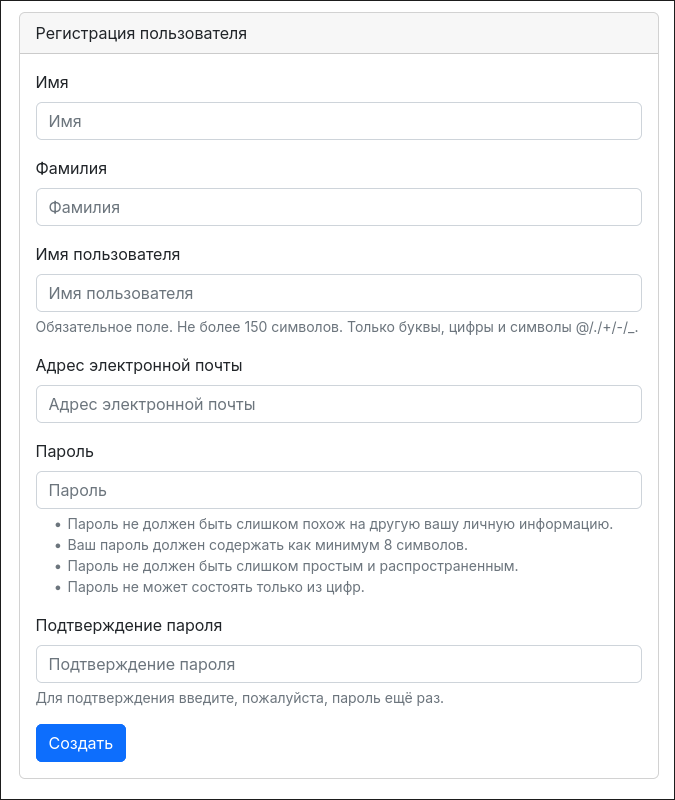
\includegraphics[width=0.8\textwidth]{static/register.png}
    \caption{Форма для регистрации пользователя}
    \label{fig:registration}
\end{figure}

\begin{figure}[H]
    \centering
    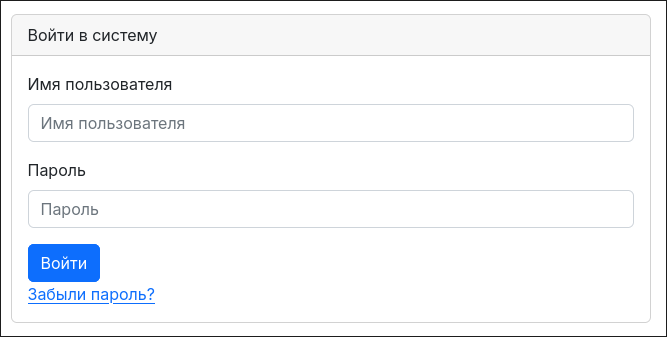
\includegraphics[width=0.8\textwidth]{static/login.png}
    \caption{Форма для входа в систему}
    \label{fig:login}
\end{figure}

\begin{figure}[H]
    \centering
    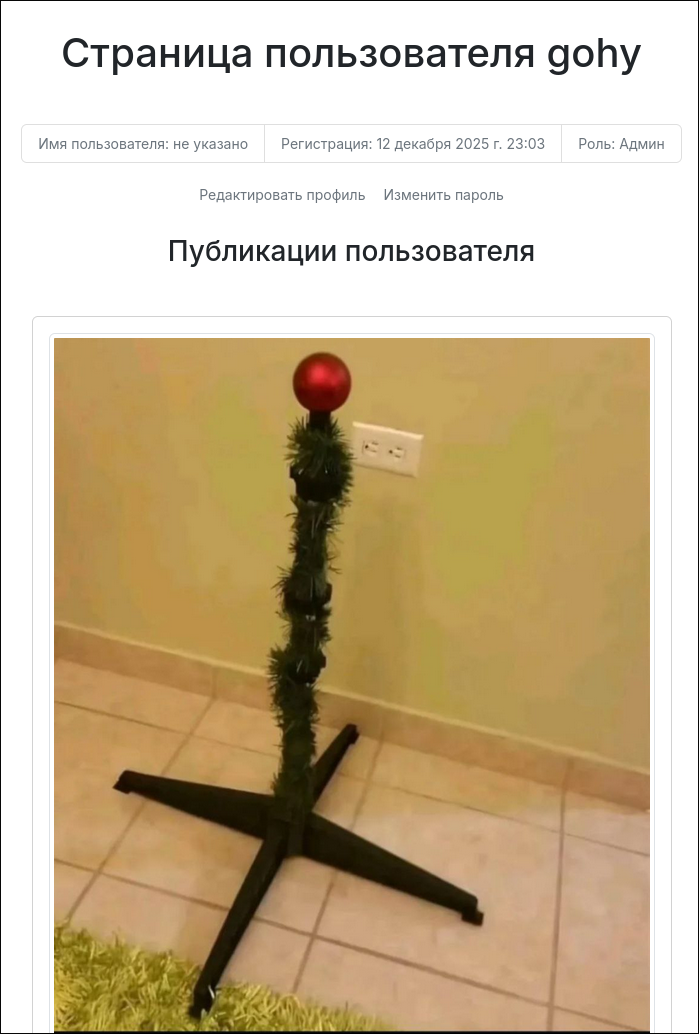
\includegraphics[width=0.8\textwidth]{static/user.png}
    \caption{Страница профиля пользователя}
    \label{fig:profile}
\end{figure}

\begin{figure}[H]
    \centering
    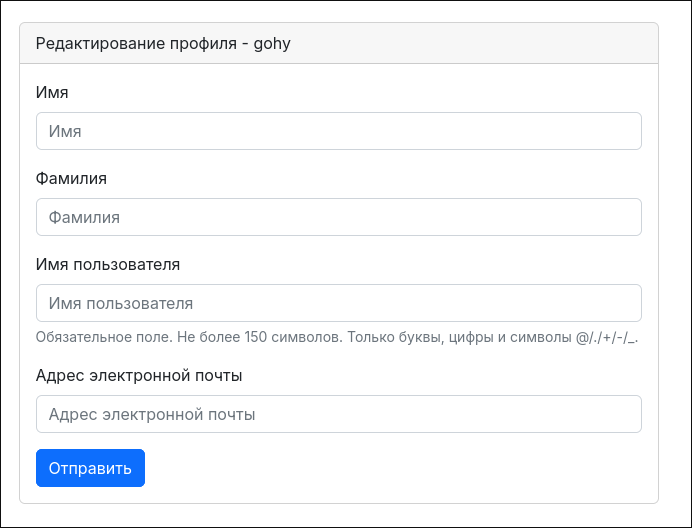
\includegraphics[width=0.8\textwidth]{static/user_edit.png}
    \caption{Страница редактирования профиля пользователя}
    \label{fig:profile_edit}
\end{figure}

\newpage
\subsection{Пагинация}

В проекте настроена пагинация на главной странице, странице пользователя и странице категории. 
Списки публикаций делятся на страницы по 10 элементов с помощью объекта \texttt{Paginator}. 
Номер страницы, которую нужно показать пользователю, передается через GET-параметр \texttt{page}.

\begin{lstlisting}
def paginate_queryset(request, queryset, per_page=10):
    paginator = Paginator(queryset, per_page)
    page_number = request.GET.get('page')
    return paginator.get_page(page_number)
\end{lstlisting}

\begin{figure}[H]
    \centering
    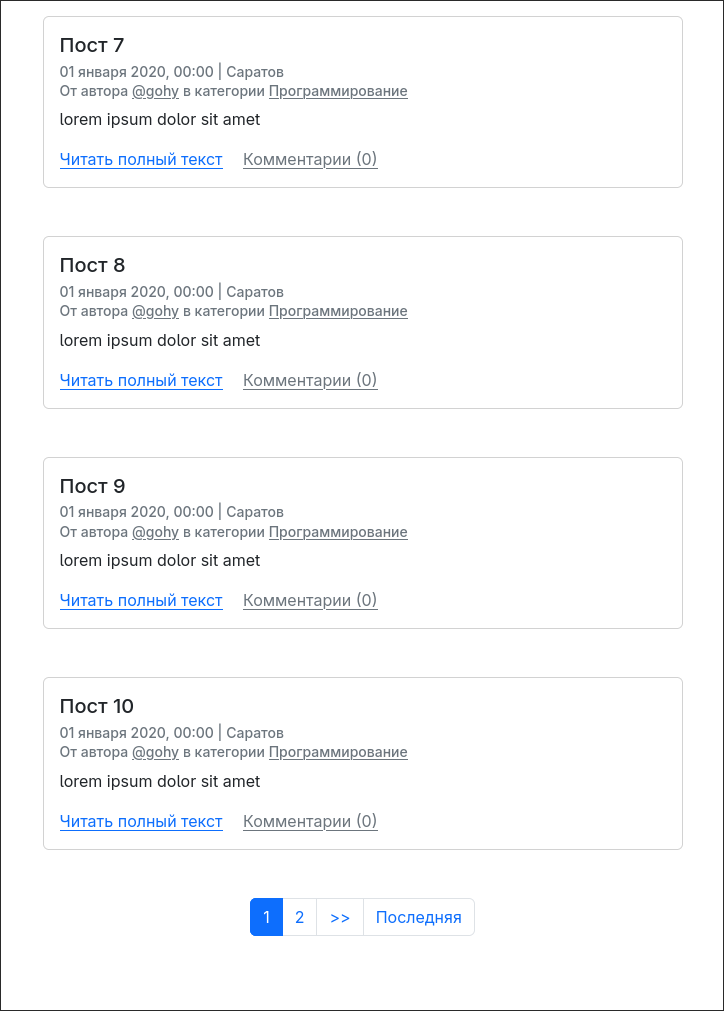
\includegraphics[width=0.9\textwidth]{static/user_pagination.png}
    \caption{Пагинация постов пользователя}
    \label{fig:user_pagination}
\end{figure}

\begin{figure}[H]
    \centering
    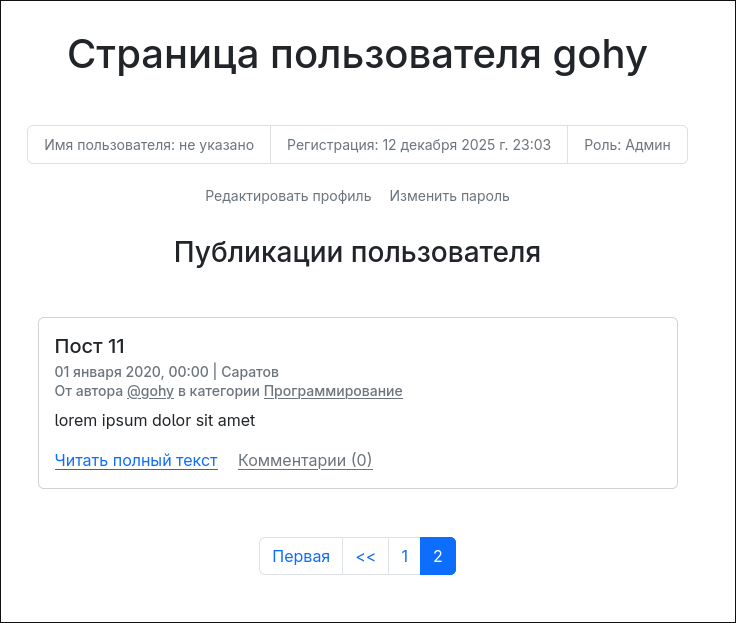
\includegraphics[width=0.9\textwidth]{static/user_pagination_2.png}
    \caption{Пагинация постов пользователя}
    \label{fig:user_pagination}
\end{figure}

На рисунках 5--6 представлена страницы пользователя с пагинацией его публикаций в размере 10 публикаций на страницу.
Блок публикации на пользовательской странице представляет собой заголовок публикации, его описание, информацию об авторе, категорию, место и время публикации. 
С помощью навигационной панели внизу страницы пользователь может перемещаться между страницами.

Пагинация реализована с помощью встроенного Django Paginator, который автоматически вычисляет количество страниц для отображения пользователю и предоставляет удобный интерфейс для навигации. 
На каждой странице отображается не более 10 публикаций, это значение можно легко поменять в главной функции, обрабатывающей пагинацию.


\newpage
\subsection{Изображения к постам}

В проекте реализована возможность добавления изображений в публикацию.
Добавлено поле \texttt{image} в модель \texttt{Post}, настроена работа с файлами.
Поле \texttt{ImageField} в модели \texttt{Post} даёт возможность пользователям загружать свои изображения.
Файлы по умолчанию сохраняются в директории \texttt{media/}, указанной в настройках проекта.
Изображения отображаются в шаблонах через тег \texttt{\{\{ post.image.url \}\}}.

\begin{lstlisting}
image=models.ImageField('
\end{lstlisting}
%image=models.ImageField("Картинка", upload_to="posts_images", blank=True)
\signatureline

\end{document}
